\documentclass[11pt]{article}

% ---------------------------------------------------------------------------
% On the Difficulty of Computing the n-th Prime
% A self-contained arXiv-style survey.
% NOTE: no TeX toolchain was available in the authoring environment, so this
% file was not compiled locally. It targets a standard TeX Live installation.
% ---------------------------------------------------------------------------

\usepackage[T1]{fontenc}
\usepackage[utf8]{inputenc}
\usepackage{lmodern}
\usepackage[margin=1in]{geometry}
\usepackage{amsmath,amssymb,amsthm,mathtools}
\usepackage{booktabs}
\usepackage{array}
\usepackage{enumitem}
\usepackage{xcolor}
\usepackage{tikz}
\usetikzlibrary{positioning,arrows.meta,decorations.pathreplacing}
\usepackage[most]{tcolorbox}
\usepackage{microtype}
\usepackage[hidelinks]{hyperref}

% ---- colors -------------------------------------------------------------
\definecolor{accent}{RGB}{30,70,120}
\definecolor{warn}{RGB}{150,40,40}
\definecolor{boxbg}{RGB}{245,247,250}

% ---- theorem environments ----------------------------------------------
\theoremstyle{plain}
\newtheorem{theorem}{Theorem}[section]
\newtheorem{proposition}[theorem]{Proposition}
\newtheorem{lemma}[theorem]{Lemma}
\newtheorem{corollary}[theorem]{Corollary}
\theoremstyle{definition}
\newtheorem{definition}[theorem]{Definition}
\newtheorem{observation}[theorem]{Observation}
\newtheorem{claimm}[theorem]{Claim}
\theoremstyle{remark}
\newtheorem{remark}[theorem]{Remark}

% ---- evidentiary-status tag --------------------------------------------
% Every nontrivial assertion is tagged with how strongly it is supported.
\newcommand{\stat}[1]{\quad\textnormal{\footnotesize\textsf{[\textcolor{accent}{#1}]}}}
\newcommand{\statline}[1]{\textnormal{\footnotesize\textsf{[\textcolor{accent}{#1}]}}}

% ---- math macros --------------------------------------------------------
\DeclareMathOperator{\li}{li}
\DeclareMathOperator{\Li}{Li}
\DeclareMathOperator{\polylog}{polylog}
\DeclareMathOperator{\Var}{Var}
\DeclareMathOperator{\rank}{rank}
\newcommand{\eps}{\varepsilon}
\newcommand{\Rinv}{R^{-1}}
\newcommand{\chiP}{\chi_{P}}
\newcommand{\Otil}{\widetilde{O}}
\newcommand{\Ztil}{\widetilde{\Theta}}
\newcommand{\Lpi}{\mathcal{L}_{\pi}}
\newcommand{\NP}{\mathsf{NP}}
\newcommand{\coNP}{\mathsf{coNP}}
\newcommand{\sharpP}{\#\mathsf{P}}
\newcommand{\NC}{\mathsf{NC}}
\newcommand{\TC}{\mathsf{TC}^{0}}
\newcommand{\Lclass}{\mathsf{L}}
\newcommand{\GapL}{\mathsf{GapL}}
\newcommand{\PP}{\mathsf{PP}}

% ---- a reusable "claims box" -------------------------------------------
\newtcolorbox{claimbox}[1]{
  enhanced, breakable, colback=boxbg, colframe=accent,
  fonttitle=\bfseries, title=#1, boxrule=0.6pt, arc=2pt,
  left=6pt, right=6pt, top=4pt, bottom=4pt}

% ---- title --------------------------------------------------------------
\title{\bfseries On the Difficulty of Computing the $n$-th Prime:\\[2pt]
\large A Catalogue of Barriers, a Computation--Verification Dichotomy,\\
and Structural Measurements}

\author{The Prime Research Project\thanks{This manuscript is a synthesis of an
extended, autonomous research effort that proceeded as a continuous loop of
falsification-first experiments. Every quantitative claim is backed by code and
a results file in the project repository; see the Methodology section
(\S\ref{sec:methodology}) for how the work was produced and for its limitations,
including the absence of external peer review.}}

\date{\today}

\begin{document}
\maketitle

\begin{abstract}
We study the problem of computing the $n$-th prime $p(n)$---equivalently the
prime-counting function $\pi(x)$---\emph{exactly}, with the goal of an algorithm
running in time polynomial in $\log x$ (``polylog''). We report, candidly, a
negative outcome: the goal was \emph{not} achieved, and we prove no new lower
bound that rules it out. This paper is instead a structured account of why the
problem resists attack. We catalogue over $700$ distinct approaches accumulated
across the effort and observe that every one falls into exactly three failure
modes---\emph{circularity}, \emph{equivalence} to the explicit (zeta-zero)
formula, and \emph{information loss}---driven by a small set of recurring
mechanisms. We isolate the locus of difficulty as a $\mathrm{SMOOTH}+\mathrm{RANDOM}$
decomposition $p(n)=\Rinv(n)+\delta(n)$, in which the smooth term $\Rinv$ (the
inverse of the Riemann $R$-function) supplies roughly half of the digits in
polylog time, while the residual $\delta(n)$ carries only $O(\log x)$ bits of
information yet appears to require $\Theta(\sqrt{x})$ work to extract, encoding
the random-looking phases of ${\sim}\sqrt{x}$ zeta zeros. We stress that the
resulting barrier is \emph{computational}, not information-theoretic: only
$\Omega(\log x)$ is unconditionally proven. We then record the one direction that
is \emph{not} blocked---verification. Computing $\pi(x)$ is hard, but checking a
claimed value is not: we describe a working, unconditionally sound interactive
proof for exact $\pi(x)$, assembled entirely from standard tools (sum-check, GKR,
polynomial commitments), whose verifier we drive from $\Theta(x)$ to
$\Theta(x^{1/4})$ large-table work against a $\Theta(\sqrt{x})$ certificate-size
wall. Finally we collect structural measurements we believe are independently
interesting: the read-once width spectrum of the prime indicator coincides with
the Hardy--Littlewood admissible-tuple census; the prime parity sequence is
indistinguishable from random under $36$ complexity measures; and the decision
problem $[\,p(n)\le x\,]$ is a fair coin against the centred guess $\Rinv(n)$ but
a fixed bias against $\li^{-1}(n)$. Throughout we label each statement by its
evidentiary status and state what would falsify it. No claim here resolves the
headline question, which remains open.
\end{abstract}

\begin{claimbox}{What this paper does and does not claim}
\textbf{It does:}
\begin{itemize}[leftmargin=1.4em,itemsep=1pt,topsep=2pt]
  \item Organise ${>}700$ failed approaches into three failure modes and ${\approx}9$ mechanisms.
  \item Localise the hardness in the $\mathrm{SMOOTH}+\mathrm{RANDOM}$ split and quantify it with measurements.
  \item Present a working, tested, unconditionally sound interactive proof for exact $\pi(x)$.
  \item Report structural facts (width/Hardy--Littlewood census, pseudorandomness, decision geography, $\sharpP$/\textsf{SETH} framing) with falsification criteria.
\end{itemize}
\textbf{It does not:}
\begin{itemize}[leftmargin=1.4em,itemsep=1pt,topsep=2pt]
  \item Give a polylog (or any sub-$\sqrt{x}$) exact algorithm for $\pi(x)$ or $p(n)$.
  \item Prove that no such algorithm exists (only $\Omega(\log x)$ is unconditional).
  \item Claim new mathematics in the verification protocol: it composes known tools, and the polylog-verifier existence is a corollary of GKR over an \textsf{AKS} circuit.
  \item Offer any speedup for \emph{computing} $\pi(x)$; the prover pays the full cost.
\end{itemize}
\end{claimbox}

\tableofcontents
\bigskip

% =====================  BODY SECTIONS INSERTED BELOW  =====================

\section{Introduction}
\label{sec:intro}

\subsection{The problem and the target}

Let $P=\{2,3,5,7,\dots\}$ be the set of primes, let
\[
  \pi(x)=\#\{p\in P : p\le x\}
\]
be the prime-counting function, and let $p(n)$ denote the $n$-th prime, so that
$\pi(p(n))=n$. The two functions are inverse to one another in the discrete
sense, and standard bracketing (Dusart) plus binary search reduces computing
$p(n)$ to a polylogarithmic number of evaluations of $\pi(x)$
\cite{aggarwal2025,dusart2010}. We therefore treat $\pi(x)$ as the primitive
object and phrase everything in terms of it, returning to $p(n)$ only where the
distinction matters.

Write $N=\lceil \log_2 x\rceil$ for the number of bits of the argument. The
target of this project is an algorithm that computes $\pi(x)$ \emph{exactly} in
time $\polylog(x)=\mathrm{poly}(N)$ --- concretely, $p(10^{100})$ in under a
second, with $100\%$ accuracy. This is the ``binary-input'' model: the input is
$N\approx 333$ bits and a polylog algorithm runs in time polynomial in $N$. We
emphasise the model because it is the entire source of difficulty.

\begin{observation}[The model gap]
\label{obs:model}
In the \emph{unary} model (input size $x$), $\pi(x)$ is computable in
\emph{sublinear} time $O(x^{2/3})$, so it is ``easy'' relative to its input. In
the \emph{binary} model (input size $N=\log_2 x$), the same $O(x^{2/3})$ bound
is $2^{2N/3}$, i.e.\ \emph{exponential} in the input length. Every algorithm
known computes $\pi(x)$ in time exponential in $N$. The question ``is $\pi(x)\in
\mathsf{P}$ (binary model)?'' is wide open.
\stat{proven for the upper bounds; the binary-model placement is open}
\end{observation}

\subsection{The honest headline}

We did not achieve the target, and we do not prove it is impossible. The best
unconditional lower bound for computing $\pi(x)$ remains the trivial
$\Omega(\log x)$ (one must at least read the input); the best upper bounds remain
$O(x^{2/3}/\log^2 x)$ combinatorially and $O(x^{1/2+\eps})$ analytically. The gap
between $\Omega(\log x)$ and $O(x^{1/2})$ --- a gap from logarithmic to
square-root in $x$, i.e.\ from $\mathrm{poly}(N)$ to $2^{N/2}$ --- is the entire
open problem, and we leave it open. What we contribute is a map of the gap: a
classification of \emph{why} the many natural attacks fail, a quantitative
account of \emph{where} the hardness lives, and a small number of adjacent
results --- chiefly that \emph{verifying} a claimed $\pi(x)$ is not subject to the
same barrier as \emph{computing} it.

\subsection{State of the art (accepted as established)}

Table~\ref{tab:sota} collects the bounds we take as the established backdrop.
None is ours; all are standard. The combinatorial line descends from
Meissel and Lehmer through Lagarias--Miller--Odlyzko \cite{lmo1985} to
Del\'egl\`ise--Rivat \cite{delegliserivat1996} and Gourdon \cite{gourdon2001},
and underlies Walisch's \texttt{primecount}, which has reached $\pi(10^{29})$ in
practice \cite{walisch}. The analytic line is Lagarias--Odlyzko
\cite{lagariasodlyzko1987}. For $p(n)$ specifically, the current word is
Aggarwal's 2025 note \cite{aggarwal2025}: binary search over $\pi$-evaluations is
asymptotically optimal among sieve-based methods, giving
$O(\sqrt{n}\,(\log n)^4)$ unconditionally.

\begin{table}[t]
\centering
\small
\begin{tabular}{@{}llll@{}}
\toprule
\textbf{Method} & \textbf{Time} & \textbf{Space} & \textbf{Reference}\\
\midrule
\multicolumn{4}{@{}l}{\emph{Computing $\pi(x)$ --- combinatorial}}\\
Sieve of Eratosthenes & $O(x\log\log x)$ & $O(x)$ & ancient \\
Meissel--Lehmer & $O(x/\log^4 x)$ & $O(x^{1/3}/\log x)$ & 1959 \\
Lagarias--Miller--Odlyzko & $O(x^{2/3}/\log x)$ & $O(x^{1/3})$ & \cite{lmo1985} \\
Del\'egl\`ise--Rivat & $O(x^{2/3}/\log^2 x)$ & $O(x^{1/3}\log^3 x)$ & \cite{delegliserivat1996} \\
Gourdon & $O(x^{2/3}/\log^2 x)$ & $O(x^{1/3}\log^3 x)$ & \cite{gourdon2001} \\[2pt]
\multicolumn{4}{@{}l}{\emph{Computing $\pi(x)$ --- analytic}}\\
Lagarias--Odlyzko & $O(x^{1/2+\eps})$ & $O(x^{1/4+\eps})$ & \cite{lagariasodlyzko1987} \\
Lagarias--Odlyzko (low space) & $O(x^{3/5+\eps})$ & $O(x^{\eps})$ & \cite{lagariasodlyzko1987} \\[2pt]
\multicolumn{4}{@{}l}{\emph{Computing $p(n)$}}\\
Best sieve & $O(n\log n/\log\log n)$ & --- & folklore \\
Binary search $+$ combinatorial $\pi$ & $O(\sqrt{n}\,(\log n)^4)$ & --- & \cite{aggarwal2025} \\
Binary search $+$ analytic $\pi$ & $O(\sqrt{n}\,\polylog n)$ {\footnotesize(RH$+$Cram\'er)} & --- & \cite{aggarwal2025} \\[2pt]
\multicolumn{4}{@{}l}{\emph{Lower bounds}}\\
Read the input & $\Omega(\log x)$ & --- & trivial \\
PRIMES $\notin \mathsf{AC}^0,\mathsf{AC}^0[p]$ & --- & --- & \cite{allendersaks2001} \\
\bottomrule
\end{tabular}
\caption{The established landscape. The headline gap is between the
$\Omega(\log x)$ lower bound and the $O(x^{1/2+\eps})$ upper bound; no
super-logarithmic unconditional lower bound for $\pi(x)$ is known.}
\label{tab:sota}
\end{table}

\subsection{Contributions and their evidentiary status}

Because honesty about status is the point of the paper, we tag every nontrivial
statement with one of: \statline{proven, unconditional}, \statline{conditional}
(on RH, GRH, SETH, BPSW, or Hardy--Littlewood), \statline{numerical},
\statline{empirical}, \statline{conjectured}, or \statline{framing}. With that
discipline in place, our contributions are:

\begin{enumerate}[leftmargin=1.6em,itemsep=2pt]
\item \textbf{A three-mode failure taxonomy} (\S\ref{sec:taxonomy}) covering
${>}700$ catalogued approaches, with ${\approx}9$ recurring deep mechanisms and a
mechanism-by-family kill matrix. \statline{framing over empirical data}
\item \textbf{The $\mathrm{SMOOTH}+\mathrm{RANDOM}$ localisation}
(\S\ref{sec:smoothrandom}): $p(n)=\Rinv(n)+\delta(n)$, with the smooth part
polylog and recovering ${\approx}70$--$90\%$ of the bits at finite $x$
(${\to}\tfrac12$ asymptotically), and the residual carrying only
$O(\log x)$ bits but apparently $\Theta(\sqrt{x})$ to extract. We are explicit
that the barrier here is \emph{computational}, not Shannon-information-theoretic.
\statline{measured; only $\Omega(\log x)$ proven}
\item \textbf{A consolidated barrier catalogue} (\S\ref{sec:barriers}): $13$
external theorems/numerical facts and $4$ project-level synthesis ``obstruction
theorems,'' each tagged by proof status.
\item \textbf{The computation--verification dichotomy} (\S\ref{sec:verification}):
a working, unconditionally sound interactive proof for exact $\pi(x)$ built from
standard tools, with the verifier's large-table work measured down to
$\Theta(x^{1/4})$ against a $\Theta(\sqrt{x})$ certificate wall. \statline{the
protocol runs; its existence-in-principle is a known corollary, not new
mathematics}
\item \textbf{Structural measurements} (\S\ref{sec:structural}): the read-once
width spectrum of $\chiP$ equals the Hardy--Littlewood admissible-tuple census; a
$36$-measure pseudorandomness audit of the prime parity sequence; and the
decision-problem geography of $[\,p(n)\le x\,]$. \statline{numerical/empirical}
\item \textbf{A complexity-status synthesis for the language}
$\Lpi=\{(x,c):\pi(x)=c\}$ (\S\ref{sec:complexity}), including the
$\polylog\text{-}\pi \Leftrightarrow \pi\in\NC$ equivalence and a conditional
$\sharpP$/\textsf{SETH} framing. \statline{conditional/framing}
\end{enumerate}

\noindent A reader interested only in the genuine positive result should read
\S\ref{sec:verification}; one interested in ``why is this hard'' should read
\S\S\ref{sec:smoothrandom}--\ref{sec:barriers}; one interested in the
phenomenology should read \S\ref{sec:structural}.

\begin{figure}[t]
\centering
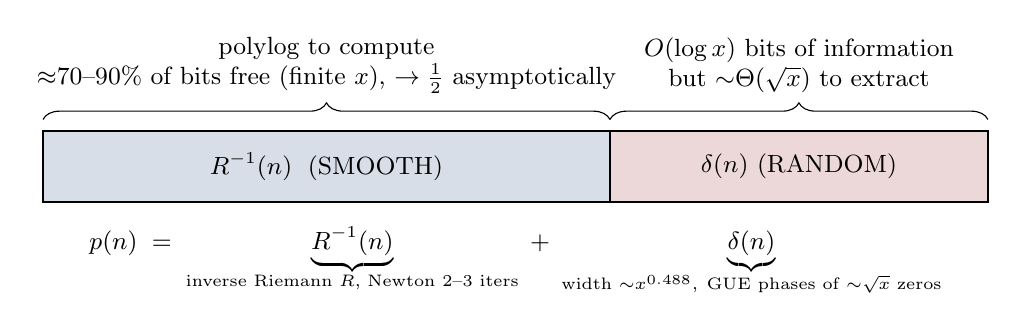
\begin{tikzpicture}[font=\small]
  % full bar
  \draw[thick] (0,0) rectangle (12,0.9);
  % smooth part
  \fill[accent!18] (0,0) rectangle (7.2,0.9);
  \fill[warn!18]  (7.2,0) rectangle (12,0.9);
  \draw[thick] (0,0) rectangle (12,0.9);
  \draw[thick] (7.2,0) -- (7.2,0.9);
  \node at (3.6,0.45) {$\Rinv(n)$ \;(SMOOTH)};
  \node at (9.6,0.45) {$\delta(n)$ (RANDOM)};
  % braces
  \draw[decorate,decoration={brace,amplitude=6pt}] (0,1.05) -- (7.2,1.05)
    node[midway,above=6pt,align=center]{polylog to compute\\${\approx}70\text{--}90\%$ of bits free (finite $x$), $\to\tfrac12$ asymptotically};
  \draw[decorate,decoration={brace,amplitude=6pt}] (7.2,1.05) -- (12,1.05)
    node[midway,above=6pt,align=center]{$O(\log x)$ bits of information\\but ${\sim}\Theta(\sqrt{x})$ to extract};
  \node[align=center] at (6,-0.75)
    {$p(n) \;=\; \underbrace{\Rinv(n)}_{\text{inverse Riemann $R$, Newton 2--3 iters}}
      \;+\; \underbrace{\delta(n)}_{\text{width } \sim x^{0.488},\ \text{GUE phases of }{\sim}\sqrt{x}\text{ zeros}}$};
\end{tikzpicture}
\caption{The $\mathrm{SMOOTH}+\mathrm{RANDOM}$ localisation of the hardness. The
smooth term is cheap and recovers most of the answer's bits; the residual is
small in \emph{information} yet expensive in \emph{computation}. Numbers are
measured (\S\ref{sec:smoothrandom}); the figure is schematic, not to scale.}
\label{fig:smoothrandom}
\end{figure}

\subsection{Provenance and a standing caveat}

The material below was produced by an extended autonomous research loop (see
\S\ref{sec:methodology}). The work has \emph{not} been externally refereed; many
measurements are at modest $N$ (we say so at each point); and several
``barriers'' we report are numerical or empirical regularities rather than
theorems. We have tried to make the status of each claim unmistakable, and to
state, for each measurement, what would falsify it. Where the project's internal
notes overclaim --- for instance by calling the central obstacle
``information-theoretic'' --- we correct the record here.

\section{The SMOOTH+RANDOM picture: where the hardness lives}
\label{sec:smoothrandom}

The single most useful organising idea the project produced is a decomposition
of the answer into a part that is cheap and a part that is expensive
(Figure~\ref{fig:smoothrandom}). It is not new mathematics --- it is the Riemann
$R$-function plus its oscillatory correction, read computationally --- but it
localises the difficulty precisely and lets us \emph{measure} it.

\subsection{The decomposition}

Let $R(x)=\sum_{k\ge 1}\frac{\mu(k)}{k}\,\li\!\big(x^{1/k}\big)$ be the Riemann
$R$-function and let $\Rinv$ be its functional inverse, so $\Rinv(n)$ is the real
$x$ with $R(x)=n$. Define the integer residual
\[
  \delta(n) \;=\; p(n) - \mathrm{round}\big(\Rinv(n)\big).
\]
Then $p(n)=\Rinv(n)+\delta(n)$ splits the $n$-th prime into a \emph{smooth}
analytic prediction and a \emph{random-looking} correction. The reason this is
the right split, rather than $\li^{-1}$ or $n\ln n$, is empirical: $R$ is the
best elementary smooth predictor of $\pi$, and (\S\ref{sec:structural}) the
decision problem $[\,p(n)\le \Rinv(n)\,]$ behaves like a fair coin while the
same test against $\li^{-1}(n)$ carries a fixed bias.

\subsection{The smooth part: \texorpdfstring{$\Rinv$}{R-inverse} is polylog and
recovers most of the bits}

Evaluating $R$ to the precision needed is polylog in $x$, and inverting it by
Newton's method is fast and \emph{scale-free}.

\begin{observation}[Smooth part is cheap]
\label{obs:smooth}
Newton iteration for $\Rinv(n)$ converges in $2$--$3$ iterations, flat across
the $22$ sampled scales ($n$ from ${\sim}200$ to ${\sim}1.2\times10^6$ tested). The
prime-count residual obeys $|\pi(x)-R(x)|\sim \sqrt{x}/\log x$ at the scales
measured, so $R$ pins down the leading bits of $\pi(x)$ for free.
\stat{numerical; matches the classical $R$-vs-$\pi$ heuristic}
\end{observation}

How many bits are ``free'' depends on $x$. Writing $B=\log_2 x$ for the bit-length
of the answer's argument and $k_0$ for the number of leading bits $R$ fixes
without help, we measured a \emph{free fraction}
\[
  k_0/B \;=\; 0.88 \longrightarrow 0.71 \quad\text{(declining as $x$ grows)},
\]
because at finite $x$ the residual $|\pi-R|$ is far below its $\sqrt{x}$
worst-case envelope (e.g.\ only ${\approx}29$ at $x=10^6$). Asymptotically the
free fraction tends to ${\approx}\tfrac12$ --- this is the sense in which ``$R$
gives about half the digits.'' We flag that the often-quoted ``${\approx}47$--$50\%$
of digits'' is the \emph{asymptotic} figure; at every finite scale we can reach,
$R$ does better ($70$--$90\%$).
\stat{numerical; the $\to\tfrac12$ limit is heuristic, tied to the $\sqrt{x}$ error law}

\subsection{The random part: small in information, expensive in computation}

The residual $\delta(n)$ is where every fast-computation attempt dies. Three
families of measurement characterise it.

\paragraph{Width.}
$\delta(n)$ has root-mean-square size growing like $\sqrt{x}$: a direct fit gives
\[
  \mathrm{RMS}\,|p(n)-\Rinv(n)| \sim x^{0.488}
\]
over $240$ values of $n$ in $8$ logarithmic bins, with the normalised error
$|\delta|/\sqrt{p(n)}$ having median $0.145$ and maximum $0.72$, and a trend in
$x$ of $-0.007\approx 0$ (i.e.\ the normalised width is bounded). This is the
$\sqrt{x}$ wall in its most elementary form.
\stat{numerical}

\paragraph{Incompressibility.}
Treated as a sequence, $\delta(n)$ resists every predictor we tried. Its entropy
rate is ${\approx}5.8$ bits/value (converged by $N=10^4$); a time-bounded
description length grows linearly, $K^t(\delta_{1..N})\approx 5.58\,N$ bits
(extensive, not compressible); the power spectrum is a featureless
$1/f^{1.70}$ continuum with no algebraic lines, and $82\%$ of Fourier modes are
needed to reconstruct it to RMSE${<}1$ (not sparsifiable). Crucially, a
transfer-entropy analysis finds $\mathrm{TE}(n\to\delta)=0.013$ bits --- the
argument $n$ contributes essentially \emph{no} information about $\delta(n)$ ---
whereas $\mathrm{TE}(\delta\to\delta)=0.051$ bits, so what little predictability
exists is purely sequential (adjacent values, autocorrelation $0.996$ at lag $1$),
useless for a single-point query. Rescaled-range/Hurst estimates ($H\approx 1.3$)
confirm a slowly drifting, random-walk-like level series.
\stat{numerical; ``no learnable structure'' is an empirical negative over the predictors tried, not a theorem}

\paragraph{Mechanism.}
This randomness is inherited from the zeta zeros. Via the explicit formula,
$\delta(n)$ encodes the accumulated phases of ${\sim}\sqrt{x}$ nontrivial zeros
$\rho$, whose local spacings follow GUE statistics
(\S\ref{sec:barriers}). The phases are the obstacle: no linear combination of
truncated partial sums predicts the next one (we revisit convergence
acceleration in \S\ref{sec:barriers}), and the number of zeros needed to settle
$\pi(x)$ exactly scales as $N_{\min}\sim x^{0.49}$ --- again $\sqrt{x}$.
\stat{numerical, resting on the (conjectural) GUE law}

\subsection{The information--computation gap (stated carefully)}

The defining feature of this problem is a gap between how much information the
answer's hard part contains and how much work it takes to produce.

\begin{proposition}[The gap, as an honest statement]
\label{prop:gap}
The residual $\delta(n)$ carries only $O(\log x)$ bits: for $x=10^{100}$,
$|\delta|\lesssim 10^{48}$, i.e.\ ${\approx}160$ bits, well under $0.15\%$ of a
$(\log_2 x)^2\approx 1.1\times10^5$-bit polylog ``budget.'' Yet every known method
to compute those bits costs $\Theta(\sqrt{x})$ (analytic, via zeros) or
$\Theta(x^{2/3})$ (combinatorial, via floor values). The only \emph{proven}
lower bound on the computation is the trivial $\Omega(\log x)$.
\stat{upper figures numerical; the $\Omega(\log x)$ is the only proven bound}
\end{proposition}

\begin{remark}[Computational, not information-theoretic --- a correction]
\label{rem:correction}
It is tempting (and the project's own early notes, and the repository's
top-level description, sometimes do this) to call this an
``information-theoretic barrier.'' That phrasing is \emph{wrong} and we correct
it. In the Shannon sense the answer is tiny --- $O(\log x)$ bits --- so there is
no information-theoretic obstruction to a short output. The barrier is purely
\emph{computational}: extracting a small number of bits appears to require
touching $\Theta(\sqrt{x})$ independent quantities. The right analogy is summing
$n$ random bits: the sum is $O(\log n)$ bits, but no method avoids reading all
$n$. Whether $\pi(x)$ truly requires super-polylog work is exactly the open
circuit-complexity question (\S\ref{sec:complexity}); nothing here proves it.
\end{remark}

This localisation also tells us what a breakthrough must do: it must compute the
$\Theta(\sqrt{x})$-fold cancellation in the zero sum (or the floor-value sum)
\emph{without} forming the summands --- a true closed form for an oscillatory
sum with GUE-random phases. The rest of the paper is, in large part, a record of
why each natural way of attempting this collapses.

\section{A taxonomy of failure}
\label{sec:taxonomy}

The project's central empirical output is negative and is best stated as a
classification. The repository catalogues, in
\texttt{status/CLOSED\_PATHS.md}, a large number of distinct attempts; its own
internal counts are inconsistent across revisions (the header reads ``$545{+}$,''
the summary table ``$641{+}$,'' and the top-level description ``$730{+}$''), so we
speak of \emph{over $700$ catalogued approaches} and treat the precise integer as
immaterial. The qualitative finding is sharp and stable: \textbf{every approach
fails in one of three ways, and the failures are driven by a short list of
recurring mechanisms.}

\subsection{Three failure modes}

\begin{definition}[The three modes]\label{def:modes}
\leavevmode
\begin{description}[leftmargin=2.2em,itemsep=2pt]
\item[\textnormal{(C) Circularity.}] The method requires primes (or a prime-indexed
object) to compute primes. The dependence is often hidden behind layers of
abstraction.
\item[\textnormal{(E) Equivalence.}] The method is a re-representation of the
explicit (zeta-zero) formula or the combinatorial sieve, and converting between
the ``spectral'' side (zeros) and the ``arithmetic'' side (primes) costs the same
$\Theta(\sqrt{x})$ or $\Theta(x^{2/3})$ as the thing it was meant to replace.
\item[\textnormal{(I) Information loss.}] The method produces a smooth
approximation that omits the $\Theta(\sqrt{x})$ ``random'' bits of
\S\ref{sec:smoothrandom}, and the gap between approximate and exact is exactly
the hard part.
\end{description}
\end{definition}

The catalogue's own mode tallies (approximate) are $\mathrm{C}\approx 82$,
$\mathrm{E}\approx 222$, $\mathrm{I}\approx 180$, with the remainder
\emph{partial}, \emph{works-but-slow}, or \emph{open}. Equivalence dominates: most
``new'' ideas turn out to be the explicit formula wearing a different coat.
\stat{empirical classification over the catalogue}

\begin{remark}[Why three suffice]
The modes are exhaustive for a structural reason. Any method either uses primes
as input ($\mathrm{C}$), or uses a transform of prime data, which is then either
faithful but no cheaper ($\mathrm{E}$) or cheaper but lossy ($\mathrm{I}$). This
is a framing, not a theorem; it earns its keep by classifying every catalogued
attempt without a leftover bin.
\stat{framing}
\end{remark}

\subsection{The recurring mechanisms}

Underneath the three modes sit a handful of concrete obstructions that do the
actual killing. We label them $\mathrm{M1}$--$\mathrm{M9}$ and use them in the
kill matrix below; each is documented in \texttt{proven/} or the catalogue.

\begin{description}[leftmargin=3.0em,itemsep=2pt]
\item[\textnormal{M1 (Explicit-formula equivalence).}] Spectral/analytic
representations reduce to $\sum_\rho x^\rho/\rho$; the spectral-to-arithmetic
conversion is the cost. \emph{(drives E)}
\item[\textnormal{M2 (The $\sqrt{x}=2^{N/2}$ wall).}] Every faithful
representation must touch $\Theta(\sqrt{x})$ independent quantities --- floor
values $\{\lfloor x/k\rfloor\}$, zeros up to height ${\sim}\sqrt{x}$, MPS bond
dimension, sieve survivors. \emph{(drives E and I)}
\item[\textnormal{M3 (Uncertainty / resolution--bandwidth).}] Smoothing kernels
(Weil, Beurling--Selberg, Gaussian, heat) cannot localise $\pi$ to $\pm\tfrac12$
without bandwidth ${\sim}\sqrt{x}$. \emph{(drives I)}
\item[\textnormal{M4 (GUE-random phases).}] Partial sums over zeros have
unpredictable phases; no convergence acceleration or recurrence predicts the next
term from a prefix. \emph{(drives E, I)}
\item[\textnormal{M5 (SMOOTH$+$RANDOM separation).}] Smooth predictors (PNT,
$R$, $\li$, Cram\'er, ML) get the polylog part; the residual is incompressible
($5.8$ bits/value, full rank). \emph{(drives I)}
\item[\textnormal{M6 (Circularity).}] Euler products, Frobenius/Chebotarev,
Mills, Wilson, cyclotomic and arithmetic-derivative encodings are indexed
\emph{by} or \emph{over} primes. \emph{(drives C)}
\item[\textnormal{M7 (Parity / sieve floor).}] Linear sieves cannot separate an
even from an odd number of prime factors (Selberg--Bombieri); inclusion--exclusion
has $2^{\pi(\sqrt{x})}$ terms and the survivor matrix is full rank. \emph{(drives I, E)}
\item[\textnormal{M8 (No-cancellation asymmetry).}] $\pi(x)$ is a positive count,
so the signed-cancellation that gives $M(x)=\sum\mu(n)$ its $O(x^{3/5})$
(Helfgott--Thompson) does not transfer. \emph{(drives E)}
\item[\textnormal{M9 (Complexity meta-barriers).}] Non-$k$-automaticity
(Mauduit--Rivat), PRIMES $\notin\mathsf{AC}^0$ (Allender--Saks--Shparlinski),
volume-law entanglement (Latorre--Sierra), the prime coding theorem
(Kolpakov--Rocke), and Natural Proofs (Razborov--Rudich) blocking lower-bound
attempts. \emph{(cross-cutting)}
\end{description}

\subsection{The mechanism-by-family kill matrix}

Table~\ref{tab:kill} maps each family of the catalogue to its dominant mode, the
mechanisms that kill it, and one representative closed entry. The pattern is that
families collapse onto a very small mechanism set: almost everything funnels into
$\mathrm{M1}/\mathrm{M2}$ (you must pay for $\sqrt{x}$ zeros or floor values) or
$\mathrm{M5}$ (your smooth model is missing the residual).

\begin{table}[t]
\centering
\footnotesize
\renewcommand{\arraystretch}{1.25}
\begin{tabular}{@{}p{2.55cm} c p{2.05cm} p{7.4cm}@{}}
\toprule
\textbf{Family} & \textbf{Mode} & \textbf{Mechanisms} & \textbf{Representative closed approach (finding)}\\
\midrule
Analytic / zeta zeros & E,I & M1,M2,M4 & Convergence acceleration of the zero sum (Richardson/Aitken/Shanks/Pad\'e/Ces\`aro): errors \emph{grow} as $N^{+1}$; GUE phases make terms independent. \\
Algebraic / $p$-adic & C,E & M1,M6 & Number-field sieve analogue: $\zeta_K$ has \emph{more} zeros than $\zeta_{\mathbb{Q}}$; harder, not easier. \\
Sieve / combinatorial & E,I & M2,M7 & Determinant/permanent sieve: reduces to M\"obius inclusion--exclusion with $2^{\pi(\sqrt{x})}$ terms; survivor matrix full rank. \\
ML / statistical & I & M5 & Unlimited decision tree: $100\%$ train, ${\approx}19\%$ test accuracy --- below majority vote. No learnable pattern. \\
Quantum & E,I & M2,M9 & Prime-state entanglement is volume-law $S\sim\tfrac{7}{8}\cdot\tfrac{n}{2}$; MPS bond dimension exponential. \\
Dynamical / automata & I & M9 & Primes are not $k$-automatic (Mauduit--Rivat); minimised DFA has $\mathrm{primorial}(y)$ states. \\
Topological / exotic & E & M1 & Prismatic cohomology / geometric Langlands: same $O(x^{1/2+\eps})$ as the analytic method. \\
Information / complexity & E,I & M2,M5 & $K^t(\delta_{1..N})\approx 5.58\,N$ bits (incompressible); sieve SVD is full rank. \\
Encoding / representation & C,I & M2,M6 & Bit-by-bit $\Delta=\pi-\li$: even the MSB needs $\Theta(\sqrt{x})$ zeros; bits entangled. \\
Additive comb.\ / Goldbach & E,I & M2,M5 & Circle-method main term is smooth (M5); the error term is the same $\sqrt{x}$ zero sum (M2). \\
Gap prediction / interp. & I & M5 & Gap entropy floor ${\approx}5.0$ bits/gap; smooth interpolation error/gap ratio ${\approx}6.5$. \\
Spectral methods & E & M1 & Selberg trace formula \emph{is} the explicit formula; Connes--Weil finds zeros but cannot sum them fast. \\
\bottomrule
\end{tabular}
\caption{Kill matrix. Families are those of \texttt{status/CLOSED\_PATHS.md};
modes from Definition~\ref{def:modes}; mechanisms $\mathrm{M1}$--$\mathrm{M9}$ as
above. The right column quotes one catalogued entry verbatim in substance.}
\label{tab:kill}
\end{table}

\subsection{Worked exemplars}

A few cases repay a closer look because they are the ones a competent
mathematician would naturally try.

\paragraph{Convergence acceleration (analytic; M1$+$M4).}
The most seductive idea is that the explicit formula's slow convergence is a
\emph{numerical} problem: truncating at $T$ zeros leaves error $O(x/T)$, so surely
Richardson or Shanks extrapolation closes the gap. It does not. The truncation
error is oscillatory with GUE-random phase, not a clean $1/N$ expansion: Richardson
beyond order $2$ diverges (condition number ${\sim}10^{3k}$), Levin/Weniger
transforms are \emph{worse} than plain summation for large $x$, and a careful
sweep finds the minimal zero count scales as $N_{\min}\sim x^{0.25\text{--}0.49}$
--- a power law, never polylog. (One genuine but bounded win: Richardson at order
$1$ on $(500,1000)$ zeros rounds $\pi(10^6)$ exactly where plain summation needs
${\sim}10^4$ zeros; this is a constant-factor, not an asymptotic, gain.)
\stat{numerical; \texttt{proven/barriers.md} items 11--12}

\paragraph{The Helfgott--Thompson non-transfer (sieve; M8).}
For the Mertens function $M(x)=\sum_{n\le x}\mu(n)$, Helfgott--Thompson reach
$O(x^{3/5})$ by exploiting the sign cancellation in $(-1)^{\omega(n)}$. One hopes
to import this to $\pi(x)$. It fails structurally: $\pi(x)$ counts $1$-almost-primes
with a \emph{positive} weight, so there is no cancellation to exploit; the
Meissel--Lehmer decomposition already \emph{is} the $\pi$-analogue of the method,
and it costs $O(x^{2/3})$. Converting $M(x)\to\pi(x)$ requires the explicit formula
($O(x^{1/2+\eps})$) anyway.
\stat{numerical; \texttt{proven/barriers.md} item 13}

\paragraph{Machine learning on the residual (statistical; M5).}
Every learner --- basis-function regression, gradient boosting, deep nets,
unbounded decision trees --- captures the smooth trend and then stalls. An
unbounded tree memorises the training primes ($100\%$) but generalises at
${\approx}19\%$, below a majority-vote baseline; basis-function regression on
$8000$ training primes matches $8/2000$ on held-out primes. This is M5 in its
purest form, and it is consistent with the prime coding theorem
(\S\ref{sec:barriers}): the sequence has ${\sim}N$ bits of time-bounded
description length, so there is no compressible formula to find.
\stat{numerical; \texttt{proven/information.md}}

\paragraph{``New algebra'' (algebraic/topological; M1$+$M6).}
Finite-field lifts ($\mathbb{F}_q\to\mathbb{Z}$ via $q\to1$), the field with one
element $\mathbb{F}_1$, $\mathbb{Z}[i]/\mathbb{Z}[\omega]$ prime counting, Artin
$L$-functions, and number-field sieves all either degenerate to the prime number
theorem (losing the residual, I) or introduce \emph{more} zeros to sum (E). The
recurring lesson: richer arithmetic objects have richer (not sparser) spectra.
\stat{empirical; catalogue ``Algebraic'' and ``Topological'' families}

\section{Proven and numerically-confirmed barriers}
\label{sec:barriers}

The failure modes of \S\ref{sec:taxonomy} are explained by a set of barriers,
some genuine theorems from the literature and some numerical regularities. We
separate the two and tag each by status. \emph{Nothing here proves the target
impossible}; collectively the barriers explain why the natural attacks die.

\subsection{External barriers}

Table~\ref{tab:barriers} lists the thirteen results the project leans on. Two
points of honesty. First, item~2 (GUE statistics) is the linchpin and it is
\emph{not} an unconditional theorem: pair correlation is known under RH in a
restricted range (Montgomery) and verified numerically to enormous height
(Odlyzko), but the full GUE law is conjectural. Several ``barriers'' below
therefore inherit a conjectural core. Second, items~11--13 are this project's own
\emph{numerical} confirmations, not theorems.

\begin{table}[t]
\centering
\footnotesize
\renewcommand{\arraystretch}{1.2}
\begin{tabular}{@{}p{3.0cm} p{8.5cm} p{1.9cm}@{}}
\toprule
\textbf{Barrier} & \textbf{Statement (abbreviated)} & \textbf{Status}\\
\midrule
1. Explicit-formula convergence & Exact $\pi(x)$ needs all zeros; truncating at $T$ leaves error $O(x/T)$, so $T>x$ for error ${<}1$ \cite{riemann1859,vonmangoldt}. & proven \\
2. GUE statistics of zeros & Local zero spacings follow GUE; zero-sum phases are random-looking \cite{montgomery1973,odlyzko1987}. & numerical / conj. \\
3. Mauduit--Rivat & The prime indicator is not $k$-automatic for any $k\ge2$ \cite{mauduitrivat2010}. & proven \\
4. PRIMES $\notin\mathsf{AC}^0$ & Primality is not in constant-depth circuits, incl.\ $\mathsf{AC}^0[p]$ \cite{allendersaks2001}. & proven \\
5. Aggarwal optimality & Binary search on $\pi$ is asymptotically optimal among sieve methods for $p(n)$ \cite{aggarwal2025}. & proven \\
6. Parity barrier & Linear sieves cannot separate even/odd $\#$prime-factors \cite{selberg,bombieri1976}. & proven \\
7. Volume-law entanglement & The prime state has $S\sim\tfrac{7}{8}\cdot\tfrac{n}{2}$; MPS bond dim is exponential \cite{latorresierra2014,garciamartin2020}. & proven (num.) \\
8. Prime coding theorem & $\mathbb{E}[K_U(\chiP{\restriction}_N)]\sim N$ bits; no compressible formula \cite{kolpakovrocke2023}. & proven \\
9. Smooth-interpolation barrier & Best smooth fit has error $O(\sqrt{p}/\ln p)\gg$ gap $O(\ln p)$; ${\approx}8/2000$ exact. & numerical \\
10. Closed-form circularity & Mills/Willans/floor-sum formulas are circular or worse than trial division. & proven \\
11. Richardson is bounded & Order-$1$ Richardson rounds $\pi(10^6)$ exactly but only saves a constant factor. & numerical \\
12. No acceleration beats $\sqrt{x}$ & No linear acceleration reduces the zero count below a power of $x$; error is oscillatory. & numerical \\
13. H--T does not transfer & $\pi(x)$'s positivity blocks the $\mu$-cancellation behind $M(x)$'s $O(x^{3/5})$. & numerical \\
\bottomrule
\end{tabular}
\caption{External barriers and their evidentiary status. ``proven (num.)'' marks
results that are theorems under a physical/model assumption but whose
project-relevant form is numerically established.}
\label{tab:barriers}
\end{table}

\subsection{Four project-level obstruction theorems (synthesis-level)}

The project also produced four ``obstruction theorems.'' We are deliberate about
their status: \textbf{these are synthesis-level analyses, not peer-reviewed
proofs.} Their rigorous cores are restatements of standard complexity facts
specialised to $\pi(x)$; their empirical parts are confirmed only for known
methods. We state them as observations.

\begin{observation}[Circuit-size / NC equivalence]
\label{obs:circuit}
Every known algorithm yields circuits of size exponential in $N=\log_2 x$
(sieve: $O(2^{2N/3})$; analytic: $O(2^{N/2+\eps})$). Moreover, by the standard
time$\leftrightarrow$circuit translation, \emph{$\pi(x)$ is computable in
$\polylog(x)$ time iff $\pi(x)\in\NC$}. The forward direction is the definition
of $\NC$-evaluation; the converse packs a $\mathrm{poly}(N)$-time algorithm into
a $\mathrm{poly}(N)$-size, $\polylog$-depth circuit.
\stat{the equivalence is a standard fact (proven); ``all known are exponential'' is empirical}
\end{observation}

\begin{observation}[Workspace-mismatch]
\label{obs:workspace}
The natural chain
$\textsf{BPSW}\Rightarrow\textsf{PRIMES}\in\Lclass\Rightarrow\pi\in\#\Lclass
\Rightarrow\pi\in\NC^2$ breaks at the second step: an $\mathsf{NL}$ machine has
only $O(\log N)$ workspace but must \emph{generate} $N$-bit candidates not present
on its input tape. Hence $\textsf{PRIMES}\in\Lclass$ and $\pi\in\NC$ are
\emph{independent}, and the sharp question is whether $\pi\in\GapL$, i.e.\ whether
there is a $\mathrm{poly}(N)$-size, logspace-uniform matrix $A(x)$ with
$\det A(x)=\pi(x)$.
\stat{synthesis; the $\#\Lclass$ obstruction and $\GapL$ reformulation are correct framing, not a new theorem}
\end{observation}

\begin{observation}[Uniformity]
\label{obs:uniformity}
Nonuniform $\mathrm{poly}(N)$-size circuits for $\pi(x)$ exist trivially (hardcode
the primes as advice); the open difficulty is \emph{uniform} construction ---
generating the comparison primes without knowing them. Consequently any
lower-bound proof must clear the Natural Proofs barrier
\cite{razborovrudich1997}: a ``natural'' distinguisher of $\pi$ from random would
contradict standard cryptographic assumptions.
\stat{synthesis, resting on standard facts}
\end{observation}

\begin{observation}[Convergence-acceleration]
\label{obs:accel}
No linear sequence-acceleration method (Richardson of any order, Levin $u/t$,
Weniger $\delta$, smoothing) reduces the zeros needed for exact $\pi(x)$ from a
power of $x$ to subpolynomial. The truncation error is an oscillatory sum with
GUE-random phases, not a $1/N$ expansion; Richardson beyond order $2$ diverges by
condition-number blow-up, and Levin/Weniger (built for alternating series) do
\emph{worse} than plain summation.
\stat{numerical, robust across $6{+}$ methods and $x\le10^6$}
\end{observation}

These four converge on one statement: the obstacle is the \emph{uniform
aggregation} of $\Theta(\sqrt{x})$ quantities, and ruling it out would require
circuit lower bounds beyond current technique while achieving it would place a
natural problem in $\NC$. That is the precise sense in which the problem ``sits at
the frontier.''

\section{What is not blocked: computation versus verification}
\label{sec:verification}

Every barrier in \S\ref{sec:barriers} constrains \emph{computing} $\pi(x)$ from
scratch. None constrains \emph{checking} a value supplied by a prover who did the
work. This asymmetry is the project's one clean positive, and the section is
careful about what is and is not new in it.

\subsection{The dichotomy}

The decision problem $[\,\pi(x)\ge c\,]$ is, in the worst case, as hard as
computing $\pi(x)$ (binary search reduces $p(n)$ to it). Yet a prover who has run
a sieve can \emph{convince} a verifier of the exact value far more cheaply than
the verifier could recompute it. Formally we study the language
\[
  \Lpi = \{(x,c) : \pi(x)=c\},
\]
and ask for its \emph{verification} complexity rather than its computation
complexity. This appears to be the first treatment of $\pi$ from this angle.
\stat{framing; the asymmetry itself is standard IP/VC, the target is new}

\subsection{The protocol stack}

We build an interactive proof for exact $\pi(x)$ on top of the Lucy--Hedgehog
sieve recurrence
\[
  S_i(v) = S_{i-1}(v) - [\,v\ge p_i^2\,]\cdot\big(S_{i-1}(\lfloor v/p_i\rfloor)-(i-1)\big),
\]
checking each of the $K=\pi(\sqrt{x})$ layers by a low-degree sum-check. Two
structural facts make it work.

\begin{enumerate}[leftmargin=1.6em,itemsep=2pt]
\item \textbf{The sieve is built from small automata.} The multilinear extension
of the \emph{primality} indicator is dense ($2^{n/2}$ coefficients --- this is
why sum-check \emph{for computing} $\pi$ died), but the Lucy recurrence contains
no primality predicate: $\lfloor v/p\rfloor$ is a $p$-state long-division
automaton and $[\,v\ge p^2\,]$ a $3$-state comparator, each with an MLE evaluable
in $O(n\cdot W)$ by a transfer-matrix DP. Factoring primality \emph{through the
recursion} makes it verification-friendly.
\item \textbf{The correction scalar is public.} Since $S_{i-1}(p_i-1)=i-1$, each
layer chains with only two point-claims and no auxiliary prover claim.
\end{enumerate}

\begin{table}[t]
\centering
\footnotesize
\begin{tabular}{@{}lllll@{}}
\toprule
\textbf{Layer} & \textbf{Verifies} & \textbf{Verifier} & \textbf{Prover} & \textbf{Status}\\
\midrule
Wheel sum-check & $\Phi(x,\text{wheel})$ & $\polylog$ & $\Otil(x)$ & $100/100$ cheaters rejected \\
Lucy base & exact $\pi(x)$ & $\Otil(x/\log x)$ & $\Otil(x^{3/2})$ & $\pi(2^{20}{-}1){=}82025$; $50/50$ rejected \\
Lucy $+$ delegated wiring & exact $\pi(x)$ & $\Otil(\sqrt{x})$ & $\Otil(x^{3/2})$ & crossover $p{\approx}130$ \\
$+$ compressed prover, PCS & exact $\pi(x)$ & $\Otil(\sqrt{x})$ & $\Otil(x)$ & end-to-end; reach $x{\approx}6.7\times10^7$ \\
GKR-over-AKS & exact $\pi(x)$ & $\polylog$ & $\mathrm{poly}(x)$ & literature corollary; impractical constants \\
\bottomrule
\end{tabular}
\caption{The verification stack. All rows are unconditionally sound except the
PCS-based large-table compression (a hash/random-oracle assumption). The final
row is not ours: it is the standard observation that GKR over a data-parallel
$\mathsf{AKS}$ circuit already gives a polylog-verifier IP --- existence is a
\emph{corollary}, not a contribution.}
\label{tab:stack}
\end{table}

\subsection{What we measured}

\begin{proposition}[A working, sound verifier for exact $\pi(x)$]
\label{prop:verifier}
There is an implemented, unconditionally sound interactive proof for exact
$\pi(x)$ with prover work $\Otil(x)$ and verifier work $\Otil(\sqrt{x})$, with
soundness error $\le 7nK/q$ over a prime field $\mathbb{F}_q$ ($n=\log_2 x$,
$K=\pi(\sqrt{x})$). Under a collision-resistant hash (Fiat--Shamir of a
Ligero/Brakedown tensor commitment), the verifier's \emph{large-table} work drops
to $\Otil(x^{1/4})$, while total verification stays $\Theta(\sqrt{x})$ because the
certificate itself has that size.
\stat{built and tested; soundness unconditional except the PCS layer}
\end{proposition}

Concretely (demonstration field $q=2^{31}-1$, soundness ${\approx}10^{-6}$ at
$n=16$; lifted to $q=2^{61}-1$ and to generic large primes for bigger $x$):
\begin{itemize}[leftmargin=1.4em,itemsep=2pt]
\item $\pi(65535)=6542$, $\pi(262143)=23000$, $\pi(1048575)=82025$ all verified
exactly through their sieve layers; the verifier ran in $69\,\mathrm{ms}\to0.9\,\mathrm{s}$
as $x$ grew $16\times$, with $28$--$110$\,KB transcripts.
\item The verifier's large-table exponent dropped in two measured steps,
$\Theta(x)\to\Theta(\sqrt{x})\to\Theta(x^{1/4})$ (fitted slopes $1.0\to0.50\to0.26$;
Figure~\ref{fig:staircase}).
\item Reach: the full compressed chain verified $\pi(2^{26}-1)=3\,957\,809$ at
$x\approx6.7\times10^7$, with the claimed value matching an independent
from-scratch Eratosthenes sieve (prover wall ${\approx}3.6$\,h, allocation-bound).
\item Adversarial: self-consistent cheating provers --- including ones that
corrupt a DP entry and recompute all downstream layers coherently, forge an
opening, or tamper a codeword --- were rejected in every trial.
\end{itemize}
\stat{numerical, reproducible from the repository logs}

\begin{figure}[t]
\centering
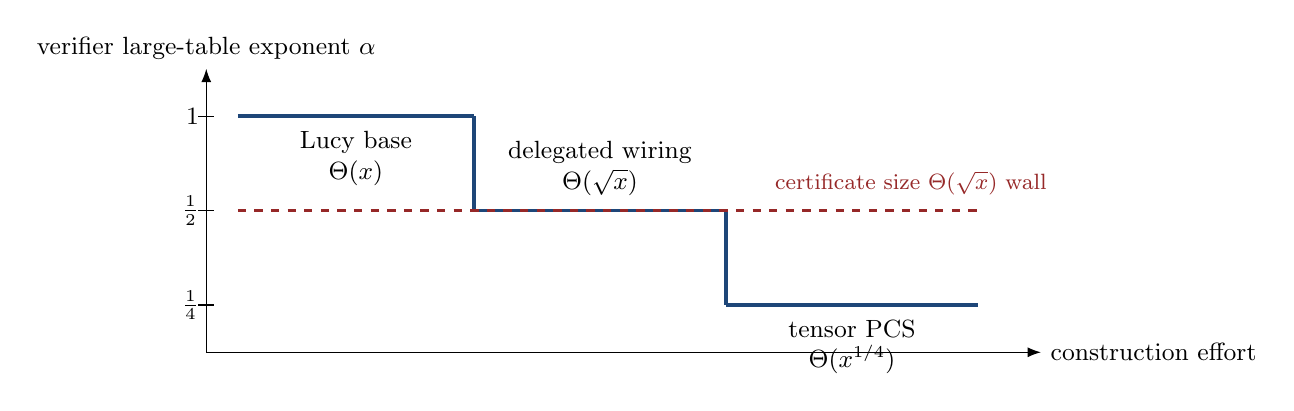
\begin{tikzpicture}[font=\small,>=Latex]
  \draw[->] (0,0) -- (10.6,0) node[right]{construction effort};
  \draw[->] (0,0) -- (0,3.6) node[above]{verifier large-table exponent $\alpha$};
  \foreach \y/\l in {0.6/{$\tfrac14$},1.8/{$\tfrac12$},3.0/{$1$}}
    \draw (-0.1,\y) -- (0.1,\y) node[left=2pt]{\l};
  % staircase
  \draw[very thick,accent]
    (0.4,3.0) -- (3.4,3.0)
    (3.4,3.0) -- (3.4,1.8)
    (3.4,1.8) -- (6.6,1.8)
    (6.6,1.8) -- (6.6,0.6)
    (6.6,0.6) -- (9.8,0.6);
  \node[align=center,below=2pt] at (1.9,3.0) {Lucy base\\$\Theta(x)$};
  \node[align=center,above=2pt] at (5.0,1.8) {delegated wiring\\$\Theta(\sqrt{x})$};
  \node[align=center,below=2pt] at (8.2,0.6) {tensor PCS\\$\Theta(x^{1/4})$};
  % cert wall
  \draw[dashed,warn,thick] (0.4,1.8) -- (9.8,1.8);
  \node[warn,right] at (7.1,2.15) {\footnotesize certificate size $\Theta(\sqrt{x})$ wall};
\end{tikzpicture}
\caption{The verifier-exponent staircase. Engineering drives the large-table
verifier work down to $\Theta(x^{1/4})$, but the certificate size itself is a
$\Theta(\sqrt{x})$ floor (dashed): \emph{total} verification cannot beat $\sqrt{x}$
without compressing the $K=\pi(\sqrt{x})$ sequential layer reductions.}
\label{fig:staircase}
\end{figure}

\subsection{The certificate wall, and why it is the same wall}

Pushing total verification below $\sqrt{x}$ requires shrinking the certificate.
We measured its size at $\alpha=0.473$ ($\Theta(\sqrt{x})$), dominated by the
$K=\pi(\sqrt{x})$ \emph{sequential} outer layer reductions; every batchable
(independent) witness is already polylog. Two findings make this a genuine wall,
not an artifact:
\begin{itemize}[leftmargin=1.4em,itemsep=2pt]
\item \textbf{Layering-inherent (construction).} Merging $j$ consecutive layers
does not drop the exponent below $0.5$ in either a direct or a fully-batched
reduction; the cost just moves between transcript, verifier work, and prover
fill ($\to x^{3/2}$ as $j\to\log K$). A sub-$\sqrt{x}$ certificate cannot come
from merging layers.
\item \textbf{Information-forced (lower bound, for this class).} The $K$ sieve
checkpoints $\{\varphi(x,a)\}$ are integer-independent: the residual matrix
against any polylog smooth predictor is full rank ($\mathrm{rank}/K\to0.97$),
so their joint information is $\Theta(\sqrt{x})\cdot\polylog$. Hence the
$\sqrt{x}$ certificate is information-forced for \emph{any sieve-reconstructing}
verifier. (A single $\pi(x)$ value is still $O(\log x)$ bits; the barrier is
joint across layers.) A fundamentally different witness is not ruled out --- that
routes through the $\sharpP$-hardness question of \S\ref{sec:complexity}.
\end{itemize}
The certificate-size wall, the verifier-work wall, and the prover-time wall are
the same $\lfloor v/p\rfloor$-semigroup wall on three faces.
\stat{numerical; the ``information-forced'' claim is proven only for the sieve-reconstruction class}

\subsection{Honest scope}

We are explicit about the limits of this result, because it is easy to oversell.
\begin{itemize}[leftmargin=1.4em,itemsep=2pt]
\item \textbf{No computation speedup.} The prover pays the full $\Otil(x)$ sieve
cost; verification being cheap does not make $\pi(x)$ cheap. This is an
adjacent-problem positive: computation unchanged, \emph{trust} exponentially
cheaper (a kilobyte-scale transcript replaces months of independent recomputation
for record $\pi(x)$ values).
\item \textbf{Standard tools.} The protocol composes LFKN sum-check
\cite{lfkn1992}, GKR-style layer reductions \cite{gkr2015}, CMT prover techniques
\cite{cmt2012}, and a Ligero/Brakedown tensor commitment
\cite{ligero2017,brakedown2023}. The genuinely new ingredients are narrow: the
\emph{target} (no prior verification protocol for $\pi$), the automaton-MLE
treatment of the sieve wiring, and the public-scalar observation.
\item \textbf{Existence is a corollary.} That a \emph{polylog}-verifier IP exists
at all is immediate from GKR over a uniform $\mathsf{AKS}$ circuit; we claim no
novelty there, only a practical $\Otil(\sqrt{x})$ verifier and the measured
walls. An earlier draft's ``polylog or $\sqrt{x}$ floor?'' question is resolved:
polylog in principle, $\sqrt{x}$ in any sieve-reconstructing construction.
\item \textbf{Unconditional vs.\ assumed.} The $\Otil(\sqrt{x})$ verifier is
information-theoretically sound; only the $x^{1/4}$ large-table compression
assumes a hash/random oracle.
\end{itemize}

\section{Structural measurements}
\label{sec:structural}

Beyond the negative catalogue, the project produced phenomenology we find
genuinely interesting --- facts about the prime indicator that are crisp,
measured, and (to our knowledge) not previously assembled. We present three.
All are \statline{numerical/empirical}; we are explicit about what they do
\emph{not} prove.

\subsection{The prime parity sequence is pseudorandom under 36 measures}

Let $\chiP(m)=[\,m\in P\,]$ and consider $\pi(x)\bmod 2$ as a Boolean function of
$N=\log_2 x$ bits (with its smooth-removed companion $f(x)=\pi(x)-R(x)$). The
project ran $36$ independent complexity measures on it --- algebraic, communication,
approximation-theoretic, spectral, information-theoretic, and circuit-synthesis ---
and in \emph{every} case the function lands within the band expected of a random
function on $N$ variables. A representative slice is Table~\ref{tab:pseudo}.

\begin{table}[t]
\centering
\footnotesize
\begin{tabular}{@{}p{6.6cm} l l@{}}
\toprule
\textbf{Measure} & \textbf{$\pi(x)\bmod 2$} & \textbf{Random}\\
\midrule
GF(2) ANF sparsity (nonzero monomials) & $0.5000$ ($N\le20$) & $0.50$ \\
Approximate degree ($\ell_\infty$, $\eps{=}0.49$) & $\lceil N/2\rceil$ & $N/2$ \\
$2$-party communication matrix rank & $2^{N/2-1}{+}2$ & $2^{N/2}$ \\
PTF degree (LP-verified) & $N/2$ & $N/2$ \\
LFSR / linear complexity & $N/2$ & $N/2$ \\
OBDD size & $2^{0.72N}$ & $2^{0.80N}$ \\
Entropy rate of $\delta(n)$ & $5.8$ bits & ${\approx}6$ \\
Power spectrum of $\delta(n)$ & $1/f^{1.69}$, no lines & no structure \\
Truth-table gzip ratio \emph{(the lone deviation)} & $2.0$--$2.6\times$ & $1.0\times$ \\
\bottomrule
\end{tabular}
\caption{Nine of the $36$ measures (full list in the source). The only deviation
from random, gzip-compressibility, is explained by the trivial density bias
($1/\ln x$ creates long zero-runs) and carries no exploitable circuit structure.}
\label{tab:pseudo}
\end{table}

\begin{observation}[The $N/2$ phase transition]
\label{obs:n2}
Five measures of different type --- approximate degree, communication rank, PTF
degree, LFSR length, and the per-bit $R$-correlation crossover --- independently
place a sharp threshold at $N/2$. This is the Boolean-complexity shadow of
\S\ref{sec:smoothrandom}: the top $N/2$ bits are the smooth $\Rinv$ part, the
bottom $N/2$ are the GUE-random residual.
\stat{numerical, $N\le 20$}
\end{observation}

\begin{remark}[A hard limit on what this can mean --- Natural Proofs]
\label{rem:natural}
This is strong \emph{indirect} evidence, and it is essential to say what it
\emph{cannot} do. Each of the $36$ measures is a \emph{natural} property in the
Razborov--Rudich sense \cite{razborovrudich1997} (efficiently computable on truth
tables, satisfied by most functions). Hence \emph{no amount} of such evidence can
prove $\pi(x)\bmod2$ has no small circuits: a successful ``natural'' proof would
break standard cryptographic generators. Pseudorandom is also not the same as
hard --- cryptographic PRGs pass every efficient test yet have small circuits.
And all measurements are at $N\le 20$. The honest reading: $\pi(x)\bmod2$
\emph{behaves} like a pseudorandom function, but proving it \emph{is} hard is
equivalent to an unconditional circuit lower bound.
\end{remark}

\subsection{The read-once width spectrum \emph{is} the Hardy--Littlewood census}

Reading $\chiP$ as a read-once branching program, let $W_j$ be the
($j$-th cut) Nerode width and let $D_k(x)$ be the number of distinct aligned
length-$k$ windows of $\chiP$ below $x$; then $W_j=D_k(2^n)$ with $k=2^{n-j}$. The
project measured the full profile and found a clean two-regime law.

\begin{observation}[Plateau $+$ admissibility cliff]
\label{obs:width}
$W_j=2^j$ exactly through $j=16$ (every aligned window of primes is distinct ---
the global-pseudorandom regime), then collapses. The cliff is exactly the
Hardy--Littlewood admissible-tuple census:
\[
  D_k(x) = A_k + 1,
\]
where $A_k$ is the number of admissible aligned patterns of length $k$ and the
$+1$ is the single small-prime window at the origin. The cliff depth is
$\rho^*(k)$, the maximal admissible weight ($3,5,9,16,28$ at
$k=8,16,32,64,128$) --- the functional inverse of the narrowest-admissible-$k$-tuple
diameter $H(k)$ (OEIS A008407, Hensley--Richards \cite{hensleyrichards1974}). The
middle cut is maximal, $W_{n/2}=2^{n/2}$, exceeding the project's earlier MLE rank
$2050$ at $n=12$, so that factor-$2$ deficiency is linear-algebraic, not
informational.
\stat{numerical; $D_k=A_k+1$ verified to $k=32$, $A_k$-entropy law conjectured}
\end{observation}

The census saturates as predicted ($k=8$: $14=13{+}1$; $k=16$: $107=106{+}1$;
$k=32$ converging), and the growth obeys the conjectural entropy law
$A_k=e^{(1+o(1))\pi(k)}$, with the entropy constant $\lim \log_2(A_k)/k$ measured
drifting $0.46\to0.37$ over $k=8\to32$. We could \emph{not} close the $o(1)$:
$k=128$ has $A_k\sim e^{25}$ and defeats direct enumeration, so a
transfer-matrix/generating-function count is the well-posed successor. What is
new here is the bridge: the \emph{same curve} carries the project's global
``$\chiP$ is pseudorandom'' regime (the $2^j$ plateau) and its local
``$\chiP$ is Hardy--Littlewood rigid'' regime (the cliff).
\stat{the bridge is a framing; the pieces are measured/conjectured as tagged}

\subsection{Decision-problem geography: a fair coin against the right guess}

Finally, the decision problem $[\,p(n)\le \widehat{x}\,]\Leftrightarrow
[\,\pi(\widehat{x})\ge n\,]$ has a measurable ``geography'' depending on the guess
$\widehat{x}$.

\begin{observation}[The better the guess, the fairer the coin]
\label{obs:geography}
Against the biased guess $\widehat{x}=\li^{-1}(n)$, the comparison bit is
\emph{constant} ($30/30$ in the measured range) --- the Rubinstein--Sarnak bias
\cite{rubinsteinsarnak1994}, predictable up to the Skewes scale ${\sim}10^{316}$.
Against the centred guess $\widehat{x}=\Rinv(n)$, the bit is an empirical coin
flip ($10/30$ vs $20/30$). The closer the smooth guess, the closer the residual
bit is to fair --- which is the information barrier of \S\ref{sec:smoothrandom}
restated as a decision problem: all the structure is in the smooth part, and what
remains is incompressibly balanced.
\stat{numerical}
\end{observation}

\section{Complexity status of \texorpdfstring{$\Lpi$}{L-pi}}
\label{sec:complexity}

We collect what can be said, conditionally and as framing, about the language
\[
  \Lpi=\{(x,c):\pi(x)=c\}
\]
in the binary-input length $n=\log_2 x$. We have \emph{no} unconditional
separation; the value of this section is to locate $\Lpi$ precisely and to record
two clean dichotomies. Everything here is \statline{conditional/framing}; the one
proven part is the trivial $\#\mathsf{P}$ membership.

\subsection{Upper bound and the \texorpdfstring{$\NP$}{NP}-completeness obstruction}

\begin{observation}[$\pi\in\sharpP$; no short \#-witness]
\label{obs:sharpP}
$\pi(x)$ counts the $n$-bit integers $m\le x$ satisfying a $\mathrm{poly}(n)$-time
predicate (primality, by AKS \cite{aks2002}), so $\pi\in\sharpP$, $\Lpi\in\mathsf{C}_{=}\mathsf{P}$,
and $\{(x,c):\pi(x)\ge c\}\in\PP$. This is folklore and is an upper bound only:
the natural \#-witness for the Legendre sieve $\varphi(x,a)$ has $2^a$ terms, i.e.\
$2^{\Theta(\sqrt{x}/\log x)}$, doubly exponential in $n$.
\stat{proven (folklore)}
\end{observation}

\begin{observation}[$\NP$-completeness would collapse the hierarchy]
\label{obs:npcollapse}
Since $\pi$ is a function, a $\mathrm{poly}(n)$ $\NP$-witness for $\pi(x)=c$
immediately yields a $\coNP$-witness for $\pi(x)\ne c$ (exhibit the true
$c'=\pi(x)$ with its witness, $c'\ne c$). Hence
$\Lpi\in\NP\Rightarrow\Lpi\in\NP\cap\coNP$, and \textbf{$\Lpi$ $\NP$-complete
$\Rightarrow\NP=\coNP$.} The open question is therefore mere $\NP$-membership ---
the existence of a $\mathrm{poly}(n)$ certificate --- not completeness.
\stat{proven implication; membership open}
\end{observation}

\subsection{The witness-size ladder}

How large must a certificate for $\pi(x)=c$ be? Every \emph{natural} family the
project could identify sits at one of three rungs (Table~\ref{tab:ladder}). Three
independent families --- the sieve transcript, the analytic/zeta witness, and the
joint-information floor --- converge at the $\sqrt{x}$ rung; enumeration sits a
full power higher; and the polylog rung is ruled out \emph{for the
sieve-reconstruction class} by the information-forcing of \S\ref{sec:verification}.
No natural witness reaches $\mathrm{poly}(n)$.

\begin{table}[t]
\centering
\footnotesize
\begin{tabular}{@{}p{8.0cm} c c@{}}
\toprule
\textbf{Witness family} & \textbf{leading power $\alpha$} & \textbf{rung}\\
\midrule
Enumeration $\NP$-cert (Pratt for each prime; a factor for each composite) & $0.985$ & $\Theta(x)$ \\
Sieve transcript (the protocol of \S\ref{sec:verification}) & $0.490$ & $\Theta(\sqrt{x})$ \\
Joint-information floor (the $\pi(\sqrt{x})$ checkpoints) & $0.486$ & $\Theta(\sqrt{x})$ \\
Zeta-zero / explicit formula (Galway $K\sim c\sqrt{x}\log^2 x$) & $0.500$ & $\Theta(\sqrt{x})$ \\
Hypothetical polylog witness (ruled out for sieve class) & $-0.000$ & $\mathrm{poly}(n)$ \\
\bottomrule
\end{tabular}
\caption{The witness-size ladder (exponents fit as
$\log\text{bits}=\alpha\log x+\delta\log\log x+c$, $k=10$--$20$). The three
nontrivial natural families agree at $\alpha\approx\tfrac12$ to within $0.014$.}
\label{tab:ladder}
\end{table}

\subsection{Why combinatorial \texorpdfstring{$\sharpP$}{\#P}-hardness is circular}

\begin{observation}[Parsimonious reduction is the goal in disguise]
\label{obs:parsimonious}
A parsimonious reduction $\#A\to\pi$ sends $w\mapsto x(w)$ with $\pi(x(w))=\#A(w)$.
To realise a target count $c$, the image must lie in $[\,p_c,\,p_{c+1}-1\,]$, so
the map $c\mapsto x(c)$ \emph{is} the inverse-prime function $p(\cdot)$ --- the
project's goal. The ``easy direction'' of the reduction is therefore as hard as
$\pi$ itself: combinatorial $\sharpP$-hardness via target-count realisation is
\emph{circular}. (The sieve instances are also lattice-structured --- sets forced
to be multiples of $d$ --- with no room to embed an arbitrary $\sharpP$-complete
count.) Consequently, if $\pi$ is $\sharpP$-hard at all, the hardness must be a
\emph{value-incompressibility} statement, not an instance embedding.
\stat{framing; precise obstruction, not a non-hardness proof}
\end{observation}

\begin{remark}[A correction to the project's own record]
An earlier project note (and \texttt{CLOSED\_PATHS.md} row 175) asserted ``exact
$\pi(x)$ is $\sharpP$-hard.'' That is an unsubstantiated claim and we retract it:
the established fact is $\pi\in\sharpP$; $\sharpP$-\emph{hardness} is open. We flag
this because the looser claim, left standing, would have implied false downstream
conclusions.
\end{remark}

\subsection{A conditional Turing-reduction barrier and a dichotomy}

\begin{observation}[SETH forbids natural Turing reductions]
\label{obs:seth}
Under SETH \cite{impagliazzopaturi2001}, no polynomial-time Turing reduction
$\#\mathsf{SAT}\to\pi$ can have query-blowup $c<c^\ast=1/\alpha$, where $\alpha$ is
$\pi$'s time exponent (measured $\alpha\approx0.66$--$0.70$ for the combinatorial
$\pi$, giving $c^\ast\approx1.5$; $\alpha=\tfrac12$ analytically gives $c^\ast=2$):
otherwise one could simulate $\pi$ by its own $x^\alpha$ algorithm and solve
$\#\mathsf{SAT}$ in $2^{o(n)}$. The natural (parsimonious) blowup is $c\to1<c^\ast$,
so every \emph{natural} Turing reduction is forbidden --- the adaptive analogue of
Observation~\ref{obs:parsimonious}.
\stat{conditional on SETH}
\end{observation}

\begin{corollary}[The exclusion dichotomy]
\label{cor:dichotomy}
Assuming $\mathsf{P}\ne\NP$, \textbf{$\pi$ computable in polylog time and $\pi$
being $\sharpP$-hard are mutually exclusive}: a polylog algorithm would put a
$\sharpP$-hard problem in (uniform) $\mathrm{poly}(n)$ time, collapsing the
hierarchy. Equivalently, \emph{a $\sharpP$-hardness proof for $\pi$ would prove the
project's goal impossible.} The two faces of the problem --- find the algorithm,
or prove hardness --- are the two ways the question can resolve, and exactly one
can hold.
\stat{conditional (P$\ne$NP); framing}
\end{corollary}

On present evidence $\Lpi$ is an $\NP$-intermediate-flavoured counting problem with
a $\Theta(\sqrt{x})$ certificate and no proven $\mathrm{poly}(n)$ one --- precisely
the status the $\Otil(\sqrt{x})$ verifier of \S\ref{sec:verification} realises from
above and the information floor pins from below.

\section{What actually runs}
\label{sec:artifacts}

To keep the paper grounded, we list the working, tested artifacts behind the
claims above (Table~\ref{tab:artifacts}). Each is a real program with a selftest
and a results file; none is a polylog exact algorithm, and we do not present any
as a contribution to the asymptotic state of the art.

\begin{table}[t]
\centering
\footnotesize
\begin{tabular}{@{}p{3.0cm} p{4.4cm} p{4.6cm} c@{}}
\toprule
\textbf{Artifact} & \textbf{Computes} & \textbf{Measured behaviour} & \textbf{Exact?}\\
\midrule
$\Rinv$ approximator & smooth prediction of $p(n)$ & Newton $2$--$3$ iters, scale-free; ${\approx}70$--$90\%$ of bits & no (smooth) \\
Lucy/Meissel $\pi(x)$ & exact $\pi(x)$ & $x^{0.66\text{--}0.70}$; ${\approx}0.3$--$2$\,ms/call (C) to $10^8$ & yes \\
Aggarwal $\times$ Dusart $\times$ BPSW & exact $p(n)$ & verified to $n=10^7$ ($p=179\,424\,673$); ${\approx}25$--$65\%$ over Aggarwal-only & yes \\
Sum-check verifier & checks exact $\pi(x)$ & $\Otil(\sqrt{x})$ verifier; reach $x\approx6.7\times10^7$ & yes (verify) \\
\bottomrule
\end{tabular}
\caption{The working artifacts. The $p(n)$ hybrid preserves Aggarwal's worst-case
$O(\sqrt{n}\log^4 n)$ and improves only the practical constant; its one regularity
is that the optimal narrowing knob obeys $K^\ast\sim\sqrt{\text{bracket width}}$ in
the fast-$\pi$ regime.}
\label{tab:artifacts}
\end{table}

The honest summary of this table is short: we can compute the \emph{smooth half}
of $p(n)$ in polylog time, we can compute $\pi(x)$ exactly only in time
$x^{2/3}$-ish, and we can \emph{verify} an exact $\pi(x)$ in $\Otil(\sqrt{x})$.
The polylog target touches none of these.

\section{Open problems and where a breakthrough must come from}
\label{sec:open}

\subsection{The central gap}

The one sentence worth repeating: the gap between the proven lower bound
$\Omega(\log x)$ and the proven upper bound $O(x^{1/2+\eps})$ --- from
$\mathrm{poly}(n)$ to $2^{n/2}$ --- is essentially unstudied for a natural problem,
and closing it in either direction is the whole question. By
Observation~\ref{obs:circuit} this is the same as asking whether $\pi(x)\in\NC$
(indeed whether it has $\mathrm{poly}(n)$-size circuits), and by
Corollary~\ref{cor:dichotomy} a hardness resolution would go through
$\sharpP$-hardness.

\subsection{Four concrete frontiers}

The project leaves four sharply-posed sub-questions, each of which is a clean
target in its own right:
\begin{enumerate}[leftmargin=1.7em,itemsep=3pt]
\item \textbf{Growing-dimension matrix powering in $\TC$.} Fixed-dimension MPOW is
in $\TC$, and $\mathbb{F}_{2^n}$ exponentiation is in $\TC$ via Frobenius
\cite{healyviola2006}, but the AKS route to PRIMES $\in\TC$ needs
\emph{growing-dimension} ($k=\polylog$) powering over $\mathbb{Z}_n$, which sits
exactly at the $\TC/\mathsf{NC}^1$ boundary and is genuinely open.
\item \textbf{$\sharpP$-hardness of $\pi$.} The sole remaining lower-bound lever
(Observation~\ref{obs:parsimonious}): if true it must be a value-incompressibility
statement, and by Corollary~\ref{cor:dichotomy} it would settle the headline
question negatively.
\item \textbf{$\GapL$ / determinantal form.} Is there a $\mathrm{poly}(n)$-size,
logspace-uniform matrix $A(x)$ with $\det A(x)=\pi(x)$ (i.e.\ $\pi\in\GapL$)? This
is the sharpest positive target (Observation~\ref{obs:workspace}); it would bypass
the workspace mismatch entirely.
\item \textbf{The sequential-sieve / layer-batching wall.} Algebraically compress
the semigroup generated by $v\mapsto\lfloor v/p\rfloor$. A sub-$\sqrt{x}$
certificate (even computational) would be new and would crack the
$\Theta(\sqrt{x})$ wall of \S\ref{sec:verification}; merging layers provably does
not suffice.
\end{enumerate}
A smaller, self-contained number-theory target also remains: closing the $o(1)$ in
the census entropy law $A_k=e^{(1+o(1))\pi(k)}$ at $k=128$ (a transfer-matrix or
generating-function count), which the direct enumeration cannot reach.

\subsection{What a breakthrough would have to be}

The localisation of \S\ref{sec:smoothrandom} says the positive direction requires
\emph{computing a $\Theta(\sqrt{x})$-fold cancellation in an oscillatory sum with
GUE-random phases without forming the summands} --- a genuine closed form where
none is known. The negative direction requires \emph{super-polynomial uniform
circuit lower bounds for an explicit function}, which must clear the Natural Proofs
barrier (Remark~\ref{rem:natural}). Both are at or beyond the current frontier of
their fields. It is entirely possible that the problem requires mathematics that
does not yet exist; nothing we found rules out a fast algorithm, and nothing we
found produces one.

\section{Methodology and honesty statement}
\label{sec:methodology}

\subsection{How the work was produced}

This material is the synthesis of a long-running \emph{autonomous} research loop:
independent cycles, each of which read a single live state document, performed one
piece of falsification-first work, and recorded the outcome before stopping. Three
disciplines shaped the corpus and are worth stating because they affect how the
results should be read:
\begin{itemize}[leftmargin=1.4em,itemsep=2pt]
\item \textbf{Catalogue-first.} Before any approach was pursued, it was checked
against the closed-paths catalogue; closing an approach meant adding a row with
its mechanism. This is why the negative results are unusually complete and why the
taxonomy of \S\ref{sec:taxonomy} has no leftover bin.
\item \textbf{Code or it didn't happen.} Each experiment is a single
CLI-parameterised script with a \texttt{--selftest} (boundary cases become
permanent regression tests) and a results file stating \emph{what would falsify
the result}. The numbers in this paper are drawn from those files and logs.
\item \textbf{Honest reporting as a hard constraint.} Failures are filed as
failures with the mechanism; earlier overclaims (including the project's own ---
the ``information-theoretic barrier'' phrasing of Remark~\ref{rem:correction}, the
``$\pi$ is $\sharpP$-hard'' assertion we retracted, the ``polylog or $\sqrt{x}$''
question we resolved) are corrected when found wrong.
\end{itemize}

\subsection{Limitations}

We list these plainly so the reader can calibrate.
\begin{itemize}[leftmargin=1.4em,itemsep=2pt]
\item \textbf{No external peer review.} The corpus has not been refereed; this
manuscript is the first attempt to expose it to outside scrutiny.
\item \textbf{Small $N$.} Many structural measurements are at $N\le 20$
($x\le10^6$) and the verifier reach is $x\approx6.7\times10^7$; asymptotic claims
extrapolate scaling fits and should be read as such.
\item \textbf{Synthesis-level ``theorems.''} The four obstruction theorems
(\S\ref{sec:barriers}) are arguments, not refereed proofs; their rigorous cores
are standard facts specialised to $\pi$.
\item \textbf{Conjectural cores.} The GUE law (and everything resting on it) is
numerical/conjectural; the $\sharpP$ and SETH statements are conditional or
framing; the census entropy law is conjectured.
\item \textbf{Novelty bar is internal.} ``Novel'' in the project sense means
``not in the catalogue and not obvious from one careful reading of the
literature''; we do not claim priority against the entire literature, and the
verification protocol explicitly composes known tools.
\end{itemize}

\section{Conclusion}
\label{sec:conclusion}

Computing $\pi(x)$ or $p(n)$ exactly in time $\polylog(x)$ remains open, and this
paper does not move the headline bounds. What it offers instead is a map. The
hardness is localised to the residual $\delta(n)=p(n)-\Rinv(n)$: small in
information ($O(\log x)$ bits), expensive in computation
($\Theta(\sqrt{x})$ apparent), and encoding the GUE-random phases of $\sqrt{x}$
zeta zeros --- a \emph{computational}, not information-theoretic, barrier. Over
$700$ catalogued attacks fail in one of three ways, driven by a short list of
mechanisms that all reduce to ``you must aggregate $\Theta(\sqrt{x})$ quantities.''
The one direction that escapes is \emph{verification}: exact $\pi(x)$ is succinctly
checkable, with a working $\Otil(\sqrt{x})$ verifier and a $\Theta(\sqrt{x})$
certificate wall we show to be information-forced for the sieve class. And the
phenomenology is sharp: the prime parity is pseudorandom under $36$ measures, its
read-once width spectrum \emph{is} the Hardy--Littlewood census, and the decision
problem is a fair coin against the right smooth guess. The problem sits exactly at
the frontier --- a fast algorithm would place a pseudorandom-looking, $\sharpP$
function in $\NC$, while proving impossibility would require circuit lower bounds
beyond current technique. We expect progress to require new mathematics, and we
have tried to say precisely which mathematics, and precisely how confident one
should be in each step along the way.

\appendix

\section{The closed-path taxonomy}
\label{app:taxonomy}

Table~\ref{tab:families} reproduces the family inventory of
\texttt{status/CLOSED\_PATHS.md} with the dominant failure mode of each.
Aggregate mode tallies (from the catalogue's own summary, ${\approx}641$
classified): circularity $\mathrm{C}\approx82$, equivalence
$\mathrm{E}\approx222$, information loss $\mathrm{I}\approx180$; the remainder are
\emph{partial} (${\approx}19$), \emph{works-but-slow} (${\approx}8$), \emph{exists
but useless} (${\approx}3$), or \emph{open} ($5$). As noted in
\S\ref{sec:taxonomy}, the catalogue's headline count drifts across revisions
($545{+}/641{+}/730{+}$); we use ``over $700$.''

\begin{table}[h]
\centering
\footnotesize
\begin{tabular}{@{}p{6.7cm} c p{4.6cm}@{}}
\toprule
\textbf{Family (catalogue heading)} & \textbf{Dominant mode} & \textbf{Typical mechanism}\\
\midrule
Analytic / explicit formula / zeta zeros & E, I & M1, M2, M4 \\
Algebraic / number theory / $p$-adic & C, E & M1, M6 \\
Sieve / combinatorial / counting & E, I & M2, M7 \\
Machine learning / statistical / fitting & I & M5 \\
Quantum computing / quantum information & E, I & M2, M9 \\
Dynamical systems / automata & I & M9 \\
Topological / exotic mathematics & E & M1 \\
Information theory / complexity theory & E, I & M2, M5, M9 \\
Encoding / novel representations & C, I & M2, M6 \\
Additive combinatorics / Goldbach / partitions & E, I & M2, M5 \\
Gap prediction / interpolation & I & M5 \\
Spectral methods & E & M1 \\
Communication / streaming / preprocessing / boosting & E, I & M2, M5 \\
\bottomrule
\end{tabular}
\caption{Catalogue families and their dominant failure mode/mechanism. Mechanisms
$\mathrm{M1}$--$\mathrm{M9}$ are defined in \S\ref{sec:taxonomy}.}
\label{tab:families}
\end{table}

\section{Selected verified edges}
\label{app:edges}

The project maintains an internal catalogue of ``edges'' (verified mathematical
facts), each graded by an internal evidence-strength tag (\textsf{EVS}:
H/M/L/shape). Table~\ref{tab:edges} lists a representative selection cited above;
the grades are the project's own and are not peer-reviewed.

\begin{table}[h]
\centering
\footnotesize
\begin{tabular}{@{}l p{10.4cm} c@{}}
\toprule
\textbf{ID} & \textbf{Statement} & \textbf{EVS}\\
\midrule
E1.1 & $E(x)=\pi(x)-\li(x)$ carries only $O(\log x)$ bits. & H \\
E1.3 & Per-bit difficulty of $p(n)$ is a sharp ${\approx}4$-bit sigmoid. & H \\
E1.4 & $N/2$ universality (degree/rank/PTF/LFSR/correlation crossover). & M \\
E2.1 & MPS bond-dimension identity at every primorial cut (wheel-$W$ gain $\phi(W)/W$). & H \\
E2.2 & Liouville/parity identity $\pi(x)=\tfrac{x-L(x)}{2}-C_3(x)$. & M \\
E3.3 & Riemann's $R(x)$ recovers ${\approx}50\%$ of the digits, exactly. & H \\
E3.4 & Spectral truncation gives a unique prime in a tiny window. & H \\
E4.4 & Telescoped (Meissel--Lehmer) parallel depth $=\pi(x^{1/3})$. & L \\
E5.1 & BPSW correctness $\Rightarrow$ PRIMES $\in\TC$. & H \\
E5.3 & Growing-dimension MPOW in $\TC$ --- the only open frontier. & H \\
E6.6 & Aggarwal 2025 binary-search optimality for $p(n)$. & H \\
E6.8 & Dusart bracketing: $p_n$ in an interval of width ${\sim}n$. & M \\
E7.1 & Zeta zeros are GUE-typical / ``independent'' to order $6$. & shape \\
\bottomrule
\end{tabular}
\caption{Selected edges from \texttt{EDGES.md}. \textsf{EVS} is the project's
internal evidence grade, not an external rating.}
\label{tab:edges}
\end{table}

\section{Reproducibility and file map}
\label{app:repro}

Every numerical claim traces to a script (with \texttt{--selftest}) and a
\texttt{*\_results.md} in the repository. The principal locations are:
\begingroup\sloppy
\begin{itemize}[leftmargin=1.4em,itemsep=1pt]
\item \texttt{proven/} --- barriers (\texttt{barriers.md}, \texttt{complexity.md},
\texttt{information.md}) and the four obstruction notes
(\texttt{circuit\_size\_barrier.md}, \texttt{uniformity\_barrier.md},
\texttt{workspace\_mismatch\_barrier.md}, \texttt{convergence\_acceleration\_barrier.md}).
\item \texttt{novel/} --- \texttt{succinct\_verification\_of\_pi.md},
\texttt{failure\_taxonomy.md}, \texttt{info\_computation\_gap.md},
\texttt{pseudorandomness\_of\_pi.md}.
\item \texttt{status/CLOSED\_PATHS.md} --- the full closed-path catalogue;
\texttt{EDGES.md} --- the verified-edge catalogue.
\item \texttt{experiments/\allowbreak constructions/\allowbreak p12\_\allowbreak sumcheck\_\allowbreak pi\_\allowbreak verification/} --- the
verification stack (\texttt{compressed\_layer.py}, \texttt{leaf\_open.py},
\texttt{pcs\_commit.py}, \texttt{sharpP\_probe.py},
\texttt{turing\_reduction\_barrier.py}, reproduction logs).
\item \texttt{experiments/analytic/} --- convergence, zero-scaling,
sparse-precision, Wasserstein, guess-comparison-oracle, and local-pattern-census
experiments.
\item \texttt{algorithms/aggarwal\_dusart\_bpsw/} --- the $p(n)$ hybrid.
\end{itemize}
\endgroup

\section{Headline constants}
\label{app:constants}

\begin{table}[h]
\centering
\footnotesize
\begin{tabular}{@{}p{8.4cm} l@{}}
\toprule
\textbf{Quantity} & \textbf{Measured value}\\
\midrule
$R$-inverse Newton iterations (scale-free) & $2$--$3$ \\
Free-bit fraction $k_0/B$ (declining in $x$) & $0.88\to0.71$ \\
Width of $\delta(n)$ & $\sim x^{0.488}$ \\
Entropy rate of $\delta(n)$ & $5.8$ bits/value \\
Time-bounded description length $K^t(\delta_{1..N})$ & ${\approx}5.58\,N$ \\
Power spectrum of $\delta(n)$ & $1/f^{1.70}$ \\
Min.\ zeros for exact $\pi(x)$ & $N_{\min}\sim x^{0.49}$ \\
Verifier large-table exponent (staircase) & $1.0\to0.50\to0.26$ \\
Certificate-size exponent & $0.473$ ($\Theta(\sqrt{x})$) \\
Verification reach & $x=2^{26}-1\approx6.7\times10^7$ \\
Pseudorandomness measures passed & $36$ \\
Census law & $D_k(x)=A_k+1$, $A_k=e^{(1+o(1))\pi(k)}$ \\
Census entropy constant $\log_2(A_k)/k$ & $0.46\to0.37$ ($k=8\to32$) \\
$p(n)$ hybrid practical gain over Aggarwal-only & ${\approx}25$--$65\%$ \\
\bottomrule
\end{tabular}
\caption{The paper's headline measured constants, with sources in
Appendix~\ref{app:repro}.}
\label{tab:constants}
\end{table}

\begin{thebibliography}{99}
\small

\bibitem{aggarwal2025} Aggarwal, \emph{A note on the complexity of computing the $n$-th prime}, arXiv:2510.16285, 2025.

\bibitem{aks2002} M.~Agrawal, N.~Kayal, N.~Saxena, \emph{PRIMES is in P}, Annals of Mathematics \textbf{160} (2004), 781--793.

\bibitem{allendersaks2001} E.~Allender, M.~Saks, I.~Shparlinski, \emph{A lower bound for primality}, Journal of Computer and System Sciences \textbf{62} (2001), 356--366.

\bibitem{bombieri1976} E.~Bombieri, \emph{The asymptotic sieve}, Rendiconti Accad.\ Naz.\ XL \textbf{1/2} (1975/76), 243--269.

\bibitem{brakedown2023} A.~Golovnev, J.~Lee, S.~Setty, J.~Thaler, R.~S.~Wahby, \emph{Brakedown: linear-time and field-agnostic SNARKs for R1CS}, CRYPTO 2023.

\bibitem{cmt2012} G.~Cormode, M.~Mitzenmacher, J.~Thaler, \emph{Practical verified computation with streaming interactive proofs}, ITCS 2012, 90--112.

\bibitem{delegliserivat1996} M.~Del\'egl\`ise, J.~Rivat, \emph{Computing $\pi(x)$: the Meissel, Lehmer, Lagarias, Miller, Odlyzko method}, Mathematics of Computation \textbf{65} (1996), 235--245.

\bibitem{dusart2010} P.~Dusart, \emph{Estimates of some functions over primes without R.H.}, arXiv:1002.0442, 2010.

\bibitem{garciamartin2020} D.~Garc\'ia-Mart\'in, E.~Ribas, S.~Carrazza, J.~I.~Latorre, G.~Sierra, \emph{The Prime state and its quantum relatives}, Quantum \textbf{4} (2020), 371.

\bibitem{gkr2015} S.~Goldwasser, Y.~T.~Kalai, G.~N.~Rothblum, \emph{Delegating computation: interactive proofs for muggles}, Journal of the ACM \textbf{62}(4) (2015), 27; orig.\ STOC 2008.

\bibitem{gourdon2001} X.~Gourdon, \emph{Computation of $\pi(x)$: improvements to the Meissel, Lehmer, Lagarias, Miller, Odlyzko, Del\'egl\`ise and Rivat method}, preprint, 2001.

\bibitem{healyviola2006} A.~Healy, E.~Viola, \emph{Constant-depth circuits for arithmetic in finite fields of characteristic two}, STACS 2006, 672--683.

\bibitem{hensleyrichards1974} D.~Hensley, I.~Richards, \emph{Primes in intervals}, Acta Arithmetica \textbf{25} (1974), 375--391.

\bibitem{impagliazzopaturi2001} R.~Impagliazzo, R.~Paturi, \emph{On the complexity of $k$-SAT}, Journal of Computer and System Sciences \textbf{62} (2001), 367--375.

\bibitem{kolpakovrocke2023} A.~Kolpakov, A.~Rocke, \emph{On the impossibility of discovering a formula for primes using AI}, arXiv:2308.10817, 2023.

\bibitem{lagariasodlyzko1987} J.~C.~Lagarias, A.~M.~Odlyzko, \emph{Computing $\pi(x)$: an analytic method}, Journal of Algorithms \textbf{8} (1987), 173--191.

\bibitem{latorresierra2014} J.~I.~Latorre, G.~Sierra, \emph{There is entanglement in the primes}, arXiv:1403.4765, 2014.

\bibitem{lfkn1992} C.~Lund, L.~Fortnow, H.~Karloff, N.~Nisan, \emph{Algebraic methods for interactive proof systems}, Journal of the ACM \textbf{39}(4) (1992), 859--868.

\bibitem{ligero2017} S.~Ames, C.~Hazay, Y.~Ishai, M.~Venkitasubramaniam, \emph{Ligero: lightweight sublinear arguments without a trusted setup}, ACM CCS 2017, 2087--2104.

\bibitem{lmo1985} J.~C.~Lagarias, V.~S.~Miller, A.~M.~Odlyzko, \emph{Computing $\pi(x)$: the Meissel--Lehmer method}, Mathematics of Computation \textbf{44} (1985), 537--560.

\bibitem{mauduitrivat2010} C.~Mauduit, J.~Rivat, \emph{Sur un probl\`eme de Gelfond: la somme des chiffres des nombres premiers}, Annals of Mathematics \textbf{171} (2010), 1591--1646.

\bibitem{montgomery1973} H.~L.~Montgomery, \emph{The pair correlation of zeros of the zeta function}, Proc.\ Sympos.\ Pure Math.\ \textbf{24} (1973), 181--193.

\bibitem{odlyzko1987} A.~M.~Odlyzko, \emph{On the distribution of spacings between zeros of the zeta function}, Mathematics of Computation \textbf{48} (1987), 273--308.

\bibitem{razborovrudich1997} A.~A.~Razborov, S.~Rudich, \emph{Natural proofs}, Journal of Computer and System Sciences \textbf{55} (1997), 24--35.

\bibitem{riemann1859} B.~Riemann, \emph{\"Uber die Anzahl der Primzahlen unter einer gegebenen Gr\"osse}, Monatsberichte der Berliner Akademie, 1859.

\bibitem{rubinsteinsarnak1994} M.~Rubinstein, P.~Sarnak, \emph{Chebyshev's bias}, Experimental Mathematics \textbf{3} (1994), 173--197.

\bibitem{selberg} A.~Selberg, \emph{On elementary methods in prime number theory and their limitations}, in Collected Papers, vol.~I, Springer, 1989.

\bibitem{vonmangoldt} H.~von Mangoldt, \emph{Zu Riemanns Abhandlung ``\"Uber die Anzahl der Primzahlen unter einer gegebenen Gr\"osse''}, J.\ Reine Angew.\ Math.\ \textbf{114} (1895), 255--305.

\bibitem{walisch} K.~Walisch, \emph{primecount: a program to count the primes below $x$}, \texttt{https://github.com/kimwalisch/primecount}, 2026.

\end{thebibliography}

\end{document}
